\documentclass[11pt]{article}
\usepackage{certmachine}
\usepackage{graphicx}
\graphicspath{{fig/}}
%% generated by tools/paper-numbers/certified-evaluation.js — do not edit (git eece01c1497a)
\newcommand{\RepoCommit}{eece01c1497a}
\newcommand{\EnvsDate}{2026-09-16}
\newcommand{\EnvsGit}{4ba347a}
\newcommand{\CorpusFacts}{104}
\newcommand{\CorpusPinned}{103}
\newcommand{\CorpusIntegers}{52}
\newcommand{\CorpusNonzero}{52}
\newcommand{\Submissions}{4{,}418}
\newcommand{\Wrong}{4{,}000}
\newcommand{\Right}{418}
\newcommand{\FamilyRows}{tolerance-interior: inside the window, outside the certificate & 1{,}649 & wrong \\
ulp-outside: the first doubles past each endpoint & 1{,}872 & wrong \\
over-truncated: the value printed to too few digits & 468 & wrong \\
control: provably right, drawn from inside the certificate & 418 & right \\
published-wrong: a value a problem thread printed & 9 & wrong \\
float-cancellation: a naive sum whose true value is 0 & 2 & wrong \\}
\newcommand{\TolList}{$1\times10^{-3}$, $1\times10^{-4}$, $1\times10^{-6}$, $1\times10^{-8}$, $1\times10^{-9}$, $1\times10^{-10}$, $1\times10^{-12}$, $1\times10^{-14}$, $1\times10^{-15}$}
\newcommand{\TolCount}{9}
\newcommand{\GraderRows}{absolute tolerance, $|v-k|<\mathrm{tol}$ & 89.5\% & 0.5\% & 10.4\% \\
relative tolerance, $|v-k|/|k|<\mathrm{tol}$ & 90.3\% & 0.5\% & 9.6\% \\
exact match, $v=k$ as a literal & 0.0\% & 24.4\% & 75.6\% \\
certificate, $\mathrm{lo}\le v\le\mathrm{hi}$ & 0.0\% & 0.0\% & 100.0\% \\}
\newcommand{\CurveRows}{$1\times10^{-3}$ & 99.4\% & 97.6\% \\
$1\times10^{-4}$ & 99.4\% & 97.6\% \\
$1\times10^{-6}$ & 99.4\% & 97.6\% \\
$1\times10^{-8}$ & 95.3\% & 95.1\% \\
$1\times10^{-9}$ & 93.6\% & 92.3\% \\
$1\times10^{-10}$ & 92.1\% & 90.6\% \\
$1\times10^{-12}$ & 88.9\% & 86.3\% \\
$1\times10^{-14}$ & 77.5\% & 78.0\% \\
$1\times10^{-15}$ & 44.4\% & 69.8\% \\}
\newcommand{\AbsFA}{89.5\%}
\newcommand{\RelFA}{90.3\%}
\newcommand{\AbsFR}{0.5\%}
\newcommand{\ExactFR}{24.4\%}
\newcommand{\ExactFA}{0.0\%}
\newcommand{\EnclFA}{0.0\%}
\newcommand{\EnclFR}{0.0\%}
\newcommand{\AbsSound}{10.4\%}
\newcommand{\ExactSound}{75.6\%}
\newcommand{\AbsFAloose}{99.4\%}
\newcommand{\AbsFAtight}{44.4\%}
\newcommand{\RelFAtight}{69.8\%}
\newcommand{\TolLoose}{$1\times10^{-3}$}
\newcommand{\TolTight}{$1\times10^{-15}$}
\newcommand{\TwiceTolTight}{$2\times10^{-15}$}
\newcommand{\WidthMedian}{$3.6\times10^{-15}$}
\newcommand{\WidthMin}{$1.56\times10^{-17}$}
\newcommand{\WidthMax}{$6.4\times10^{-3}$}
\newcommand{\RhoMedian}{562{,}949}
\newcommand{\RhoMin}{128{,}102{,}388}
\newcommand{\NarrowestId}{terra.sigmaStar}
\newcommand{\NarrowestWhat}{$\sigma^\ast = 1/(8\pi^2)$}
\newcommand{\PubFactId}{erdos852.cstar}
\newcommand{\PubValue}{0.0752403861777}
\newcommand{\PubGap}{$6.09\times10^{-13}$}
\newcommand{\PubLo}{0.075240386178309235}
\newcommand{\PubHi}{0.075240386178309582}
\newcommand{\PubWidth}{$3.47\times10^{-16}$}
\newcommand{\EnvsForgeriesPlanted}{34}
\newcommand{\EnvsForgeriesLeaked}{0}
\newcommand{\AbsFooledUlp}{1{,}696}
\newcommand{\AbsFooledInterior}{1{,}649}
\newcommand{\AbsFooledPublished}{7}
\newcommand{\PublishedCanaries}{9}
\newcommand{\UnifInstances}{12}
\newcommand{\UnifTwoD}{5}
\newcommand{\UnifNeedled}{10}
\newcommand{\UnifRazor}{2}
\newcommand{\UnifRows}{sampling K=1e3 & +1.00 & 1 & 0 & 11 & 0 & 9 \\
sampling K=1e5 & +3.00 & 3 & 0 & 9 & 0 & 7 \\
sampling + bluffed tiling & $-$6.00 & 3 & 9 & 0 & 0 & 9 \\
interval bisection (sound) & +11.25 & 11 & 0 & 0 & 1 & 0 \\
interval, 2e3-cell budget & +9.00 & 8 & 0 & 0 & 4 & 0 \\}
\newcommand{\BluffScore}{$-$6.00}
\newcommand{\SoundScore}{+11.25}
\newcommand{\BudgetAbstained}{4}
\newcommand{\BudgetScore}{+9.00}
\newcommand{\AttackRows}{c0 & wide band & absolute-tolerance & $1.0\times10^{-6}$ & yes & $5.0\times10^{-7}$ \\
c1 & narrow band & relative-tolerance & $1.0\times10^{-9}$ & yes & $5.0\times10^{-10}$ \\
c2 & tolerance under the enclosure & absolute-tolerance & $1.0\times10^{-3}$ & no & 0 \\
c3 & sound grader & enclosure & --- & no & 0 \\
c4 & razor band & absolute-tolerance & $2.1\times10^{-13}$ & yes & 0 \\
c5 & off-centre key & absolute-tolerance & $1.0\times10^{-13}$ & yes & 0 \\
c6 & empty in floating point & absolute-tolerance & $1.0\times10^{-15}$ & no & 0 \\}
\newcommand{\AttackRungs}{7}
\newcommand{\AttackRungsNone}{3}
\newcommand{\EnvsLedgerRows}{92}
\newcommand{\EnvsLedgerModels}{11}
\newcommand{\EnvsBatteryPass}{13}
\newcommand{\EnvsBatteryReds}{5}
\newcommand{\PrimeLimit}{2{,}000{,}000}
\newcommand{\PrimesCount}{148{,}932}
\newcommand{\DroppedCount}{130{,}293}
\newcommand{\DroppedPct}{87.5\%}
\newcommand{\NaiveC}{0.0752403861777419}
\newcommand{\PublishedC}{0.0752403861777}
\newcommand{\CertLo}{0.0752403861783092455893}
\newcommand{\CertHi}{0.0752403861783095651674}
\newcommand{\AgreePlaces}{11}
\newcommand{\FailPlace}{12}
\newcommand{\PublishedDigits}{13}
\newcommand{\CstarPrimes}{1{,}857{,}858}
\newcommand{\CstarPrimeLimit}{30{,}000{,}000}
\newcommand{\CstarBits}{192}
\newcommand{\CstarDigits}{22}
\newcommand{\CZeroPublished}{1.32322827686395}
\newcommand{\CZeroDigits}{61}
\newcommand{\CZeroBisections}{200}
\newcommand{\CZeroBits}{320}
\newcommand{\DropThreshold}{208{,}064}
\newcommand{\ImpostorCount}{21}
\newcommand{\ImpostorDepth}{62}
\newcommand{\ImpostorId}{A271880}
\newcommand{\ImpostorLabel}{1/5}
\newcommand{\ImpostorName}{Decimal expansion of the probability that a random real number is evil.}
\newcommand{\ImpostorPublishedDigits}{105}
\newcommand{\OeisEntries}{14{,}677}
\newcommand{\RmPrinted}{51}
\newcommand{\RmSurvive}{50}
\newcommand{\RmRefuted}{1}
\newcommand{\RmSheets}{7}
\newcommand{\SosPass}{19}
\newcommand{\SosPrograms}{3}
\newcommand{\SosWitnessX}{(3/200000,1/1000)}
\newcommand{\SosWitnessVdot}{22103/50000000000000}
\newcommand{\MmRows}{364}
\newcommand{\MmAnswered}{324}
\newcommand{\MmCertified}{115}
\newcommand{\MmRefuted}{0}
\newcommand{\MmRejected}{147}
\newcommand{\MmMalformed}{39}
\newcommand{\MmDeclined}{23}
\newcommand{\MmBudget}{40}
\newcommand{\MmCampaigns}{12}
\newcommand{\MmModels}{3}
\newcommand{\MmCorrectionRows}{90}
\newcommand{\MmCorrectionFound}{2026-08-31}
\newcommand{\ProbeN}{10}
\newcommand{\ProbeOpusDeclined}{6}
\newcommand{\ProbeSonnetDeclined}{5}
\newcommand{\ProbeHaikuDeclined}{0}
\newcommand{\ProbeOpusN}{10}
\newcommand{\ProbeSonnetN}{10}
\newcommand{\ProbeHaikuN}{10}
\newcommand{\MmOpusVtwo}{17/24}
\newcommand{\MmSonnetVtwo}{28/40}
\newcommand{\MmHaikuAll}{0/146}
\newcommand{\LoopTrajectories}{10}
\newcommand{\LoopRounds}{31}
\newcommand{\LoopCertified}{6}
\newcommand{\LoopConversions}{0}
\newcommand{\LoopMaxRounds}{8}
\newcommand{\GsmGenerated}{2026-09-21}
\newcommand{\GsmCommit}{3101c7d}
\newcommand{\PlatRevision}{e762492}
\newcommand{\TestItems}{1{,}319}
\newcommand{\TrainItems}{7{,}473}
\newcommand{\TestAnn}{4{,}282}
\newcommand{\TrainAnn}{23{,}716}
\newcommand{\TrainAnnExact}{23{,}714}
\newcommand{\TrainAnnRefused}{2}
\newcommand{\TestProse}{3{,}572}
\newcommand{\TestProseUnread}{318}
\newcommand{\TrainProse}{19{,}671}
\newcommand{\TrainProseUnread}{1{,}711}
\newcommand{\GsmClassRows}{reproduced: every annotation exact; the answer is the last annotation's value & 1{,}207 & 6{,}981 \\
answer in prose: as above, the answer being a prose equation that checks exactly & 50 & 200 \\
answer underived: no arithmetic fault; the answer is no printed value & 47 & 193 \\
rounded step: a printed step is a rounding of its exact value & 0 & 2 \\
printed step wrong: a step is wrong by more than a rounding & 2 & 24 \\
no steps: no equation of either kind is printed & 13 & 71 \\
refused: an annotation outside the calculator grammar & 0 & 2 \\}
\newcommand{\TestReproduced}{1{,}207}
\newcommand{\TestInProse}{50}
\newcommand{\TestUnderived}{47}
\newcommand{\TestNoSteps}{13}
\newcommand{\TestReach}{1{,}257}
\newcommand{\TrainReach}{7{,}181}
\newcommand{\TestReader}{60}
\newcommand{\TrainReader}{264}
\newcommand{\WrongTest}{2}
\newcommand{\WrongTrain}{24}
\newcommand{\WrongTestNotHeld}{1}
\newcommand{\WrongTrainNotHeld}{6}
\newcommand{\WrongTrainBeside}{18}
\newcommand{\TrainRounded}{2}
\newcommand{\TrainRefused}{2}
\newcommand{\PlatConsensus}{1{,}100}
\newcommand{\PlatVerified}{99}
\newcommand{\PlatRemoved}{110}
\newcommand{\PlatRevised}{10}
\newcommand{\PlatKept}{1{,}209}
\newcommand{\PlatFlagged}{219}
\newcommand{\RemovedReproduced}{103}
\newcommand{\RevisedReproduced}{9}
\newcommand{\GsmCrossRows}{consensus & 1{,}100 & 1{,}008 & 42 & 36 & 12 & 2 \\
verified & 99 & 87 & 4 & 7 & 1 & 0 \\
removed & 110 & 103 & 4 & 3 & 0 & 0 \\
revised & 10 & 9 & 0 & 1 & 0 & 0 \\}
\newcommand{\GsmWitnessRowsA}{test & 501 & 364 / 4 = 273 & 91 & 273 & yes \\
test & 1024 & \$32 - \$20 = \$300 & 12 & 300 & no \\
train & 167 & 192*100 = \$1920 & 19200 & 1920 & no \\
train & 168 & 6*2.5 = \$18.00 & 15 & 54 & yes \\
train & 198 & 6/3 = .5 & 2 & 30 & no \\
train & 224 & 4080 + 4080 / 2 = 4000 + 2040 & 6120 & 20655 & yes \\
train & 502 & 3/1 = 1 & 3 & 6 & yes \\
train & 716 & 100 * 0.75 = \$0.75 & 75 & 265 & yes \\
train & 3002 & 8*3 = 240 & 24 & 14 & yes \\
train & 3334 & \$4200+\$3000 = \$8600 & 7200 & 7200 & no \\
train & 3409 & 10 x .5 = 10 & 5 & 5 & no \\
train & 3859 & 5 * 3 = \$15,000 & 15 & 90,000 & yes \\
train & 4593 & 14 / 1 / 4 = 14 * 4 & 7/2 & 4 & no \\}
\newcommand{\GsmWitnessRowsB}{train & 4691 & 2*8 = 24 & 16 & 570 & yes \\
train & 4973 & 200*.55 = 100 & 110 & 1100 & yes \\
train & 5195 & 5 x 1/2 = 10 & 5/2 & 1 & yes \\
train & 5396 & 1 * 2 = 20 & 2 & 130 & yes \\
train & 5781 & 7+9+1+2 = \$19.50 & 19 & 78 & yes \\
train & 6256 & 10 x 1,248 = 11,480 & 12480 & 27 & yes \\
train & 6590 & 1-2 = 96 - 70 & -1 & 26 & yes \\
train & 6700 & 2 / 12 = .125 & 1/6 & 1 & yes \\
train & 6713 & 3 x (8/16) = 6 & 3/2 & 18 & yes \\
train & 6812 & 50-8 = 44 & 42 & 8 & yes \\
train & 6842 & 500/ 2/5 = 200 & 1250 & 250 & yes \\
train & 7178 & 1152/ 1,536 = .5 & 3/4 & 1 & yes \\
train & 7444 & 14*20 = 140 & 280 & 280 & no \\}
\newcommand{\GsmRoundedList}{3390 (\$10/3 = \$3, exact 10/3); 4504 (13 / 6 = 2, exact 13/6)}
\newcommand{\TestForms}{1{,}303 plain, 14 with thousands separators and 2 negative}
\newcommand{\TrainForms}{7{,}391 plain, 79 with separators and 3 negative}
\newcommand{\InspectEvalsCommit}{788f5a2}
\newcommand{\LmEvalCommit}{d6de816}
\newcommand{\InspectVersion}{0.3.266}
\newcommand{\ObsRows}{8}
\newcommand{\ObsCorrect}{6}
\newcommand{\GsmBatteryPass}{51}
\newcommand{\GsmBatteryReds}{12}
\newcommand{\GsmSeconds}{1.4}
\newcommand{\HzGenerated}{2026-09-25}
\newcommand{\HzFits}{44}
\newcommand{\HzCertified}{44}
\newcommand{\HzLive}{23}
\newcommand{\HzRunsAgents}{21}
\newcommand{\HzSiteResults}{26}
\newcommand{\HzSeconds}{120}
\newcommand{\HzLambda}{10^{-5}}
\newcommand{\HzCoefRepro}{22}
\newcommand{\HzCoefDiffer}{1}
\newcommand{\HzDifferAlias}{Claude Mythos Preview (early)}
\newcommand{\HzDifferPrinted}{5.582}
\newcommand{\HzDifferCertified}{5.583}
\newcommand{\HzDifferBoxLo}{5.582691}
\newcommand{\HzDifferBoxHi}{5.582691}
\newcommand{\HzMaxRad}{$3.6\times10^{-13}$}
\newcommand{\HzGapMin}{$9.6\times10^{-7}$}
\newcommand{\HzGapMax}{$1.8\times10^{-4}$}
\newcommand{\HzInside}{0}
\newcommand{\HzWidthMin}{$2\times10^{-11}$}
\newcommand{\HzWidthMax}{$4\times10^{-8}$}
\newcommand{\HorizonRows}{GPT-4 0314 & 2023-03-14 & 3.987 & 3.987 & $8.6\times10^{-5}$ & $-0.641$, $1.278$ & reproduced \\
GPT-4 1106 & 2023-11-06 & 4.045 & 4.045 & $4.2\times10^{-5}$ & $-0.585$, $1.18$ & reproduced \\
Claude 3 Opus & 2024-03-04 & 3.952 & 3.952 & $3.1\times10^{-6}$ & $-0.527$, $1.046$ & reproduced \\
GPT-4 Turbo & 2024-04-09 & 3.733 & 3.733 & $2.3\times10^{-5}$ & $-0.69$, $1.312$ & reproduced \\
GPT-4o & 2024-05-13 & 6.991 & 6.991 & $8.4\times10^{-5}$ & $-0.563$, $1.578$ & reproduced \\
Claude 3.5 Sonnet (Old) & 2024-06-20 & 11.394 & 11.395 & $1.1\times10^{-4}$ & $-0.501$, $1.757$ & reproduced \\
o1-preview & 2024-09-12 & 20.329 & 20.327 & $1.4\times10^{-4}$ & $-0.63$, $2.737$ & reproduced \\
Claude 3.5 Sonnet (New) & 2024-10-22 & 20.523 & 20.523 & $6.0\times10^{-6}$ & $-0.465$, $2.026$ & reproduced \\
o1 & 2024-12-05 & 38.831 & 38.832 & $2.1\times10^{-5}$ & $-0.565$, $2.983$ & reproduced \\
Claude 3.7 Sonnet & 2025-02-24 & 60.388 & 60.389 & $2.3\times10^{-5}$ & $-0.597$, $3.535$ & reproduced \\
o3 & 2025-04-16 & 119.733 & 119.733 & $9.6\times10^{-7}$ & $-0.694$, $4.791$ & reproduced \\
Claude 4 Opus & 2025-05-22 & 100.372 & 100.366 & $6.3\times10^{-5}$ & $-0.604$, $4.014$ & reproduced \\
Claude 4.1 Opus & 2025-08-05 & 100.472 & 100.472 & $2.1\times10^{-6}$ & $-0.661$, $4.393$ & reproduced \\
GPT-5 & 2025-08-07 & 202.996 & 203.013 & $8.3\times10^{-5}$ & $-0.576$, $4.417$ & reproduced \\
Gemini 3 Pro & 2025-11-18 & 224.344 & 224.326 & $8.3\times10^{-5}$ & $-0.676$, $5.279$ & reproduced \\
GPT-5.1-Codex-Max & 2025-11-19 & 223.727 & 223.715 & $5.4\times10^{-5}$ & $-0.647$, $5.048$ & reproduced \\
Claude Opus 4.5 & 2025-11-24 & 293.003 & 292.995 & $2.9\times10^{-5}$ & $-0.54$, $4.425$ & reproduced \\
GPT-5.2 & 2025-12-11 & 352.245 & 352.249 & $1.2\times10^{-5}$ & $-0.574$, $4.855$ & reproduced \\
Claude Opus 4.6 & 2026-02-05 & 718.937 & 718.807 & $1.8\times10^{-4}$ & $-0.412$, $3.912$ & reproduced \\
GPT-5.3-Codex & 2026-02-05 & 349.496 & 349.531 & $1.0\times10^{-4}$ & $-0.518$, $4.379$ & reproduced \\
Gemini 3.1 Pro & 2026-02-19 & 384.189 & 384.147 & $1.1\times10^{-4}$ & $-0.661$, $5.676$ & reproduced \\
GPT-5.4 & 2026-03-05 & 341.741 & 341.735 & $1.7\times10^{-5}$ & $-0.52$, $4.378$ & reproduced \\
Claude Mythos Preview (early) & 2026-04-07 & 1044.645 & 1044.780 & $1.3\times10^{-4}$ & $-0.557$, $5.582$ & differs \\}
\newcommand{\HzDoubling}{128.740}
\newcommand{\HzDoublingWidth}{$1.5\times10^{-9}$}
\newcommand{\HzTrendN}{14}
\newcommand{\HzSlopeWidth}{$8.9\times10^{-14}$}
\newcommand{\HzDoublingPrinted}{128.744}
\newcommand{\HzCiLo}{104.428}
\newcommand{\HzCiHi}{158.012}
\newcommand{\HzDoublingTwentyFour}{104.7}
\newcommand{\HzTrendNTwentyFour}{12}
\newcommand{\HzPostTwentyFour}{88.6}
\newcommand{\HzPostTwentyThree}{130.8}
\newcommand{\HzExcluded}{960}
\newcommand{\HzExcludedHours}{16}
\newcommand{\HzPostN}{7}
\newcommand{\HzPostRepro}{1}
\newcommand{\HzPostDiffer}{6}
\newcommand{\HzPostGapMin}{0.6}
\newcommand{\HzPostGapMax}{12}
\newcommand{\HzPostRows}{Claude Opus 4.5 & 320 [170, 729] & 293.00 & 292.99 & differs \\
GPT-5 & 214 [117, 480] & 203.00 & 203.01 & differs \\
o3 & 121 [74, 201] & 120.00 & 119.73 & differs \\
Claude 4 Opus & 101 [58, 170] & 100.00 & 100.37 & differs \\
Claude 3.7 Sonnet & 60 [32, 106] & 60.00 & 60.39 & reproduced \\
GPT-4 1106 & 3.6 [1.6, 7.5] & 4.00 & 4.04 & differs \\
GPT-4 0314 & 3.5 [1.6, 6.9] & 4.00 & 3.99 & differs \\}
\newcommand{\HzBoth}{20}
\newcommand{\HzBothGap}{$2.2\times10^{-5}$}
\newcommand{\HzHuman}{106.4}
\newcommand{\HzHumanTasks}{188}
\newcommand{\HzRuns}{24{,}008}
\newcommand{\HzRepoCommit}{52cb829}
\newcommand{\HzRepoDate}{2026-03-06}
\newcommand{\HzFetched}{2026-09-22}
\newcommand{\HzPostDate}{2026-01-29}
\newcommand{\HzSiteUpdated}{May 8, 2026}
\newcommand{\HzOwnLogs}{15}
\newcommand{\HzOwnRollouts}{180}
\newcommand{\HzOwnTasks}{18}
\newcommand{\HzOwnVerdict}{NO DATA}
\newcommand{\HzBatteryChecks}{33}
\newcommand{\HzBatteryReds}{7}
\newcommand{\HzExAlias}{Claude 3.7 Sonnet}
\newcommand{\HzExSlopeLo}{-0.5974549266701}
\newcommand{\HzExSlopeHi}{-0.5974549266681}
\newcommand{\HzExIntLo}{3.5346505939786}
\newcommand{\HzExIntHi}{3.5346505939859}
\newcommand{\HzExHLo}{60.387561330}
\newcommand{\HzExHHi}{60.387561332}
\newcommand{\HzExSite}{60.388937}
\newcommand{\HzExRad}{$6.4\times10^{-14}$}
\newcommand{\HzExCiLo}{33.0}
\newcommand{\HzExCiHi}{104.2}
\newcommand{\HzExTasks}{228}
\newcommand{\GymDate}{2026-09-16}
\newcommand{\GymGit}{4ba347a}
\newcommand{\GymFacts}{104}
\newcommand{\GymPinned}{103}
\newcommand{\GymIntegers}{52}
\newcommand{\GymTasks}{2{,}000}
\newcommand{\GymAttackable}{1{,}395}
\newcommand{\GymImpossible}{605}
\newcommand{\GymAlways}{1{,}175}
\newcommand{\GymNever}{645}
\newcommand{\GymForgeries}{1{,}366}
\newcommand{\GymLeaked}{0}
\newcommand{\GymMedianBand}{$1.0\times10^{-13}$}
\newcommand{\GymMixRows}{impossible & 25\% & 605 & 30\% \\
razor & 35\% & 453 & 23\% \\
narrow & 25\% & 664 & 33\% \\
wide & 15\% & 278 & 14\% \\}
\newcommand{\GymDialRows}{10{,}000{,}001 & 20{,}000{,}000 & $6.84\times10^{-6}$ & breakable \\
10{,}001 & 20{,}000 & $6.84\times10^{-9}$ & breakable \\
10 & 19 & $6.50\times10^{-12}$ & breakable \\
1 & 1 & $3.42\times10^{-13}$ & breakable \\
0.6 & 0.2 & $6.84\times10^{-14}$ & breakable \\
0.51 & 0.02 & $6.84\times10^{-15}$ & breakable \\
0.5001 & 0.0002 & $6.84\times10^{-17}$ & no attack exists \\
0.5 & 0 & 0 & no attack exists \\}
\newcommand{\GymDialFact}{erdos1038.upper}
\newcommand{\GymDialWidth}{$3.4\times10^{-13}$}
\newcommand{\GymGap}{0.410}
\newcommand{\GymCarefulMean}{+0.9975}
\newcommand{\GymAlwaysMean}{+0.5875}
\newcommand{\GymBaselineN}{400}
\newcommand{\GymCarefulImpossible}{128/129}
\newcommand{\PilotDate}{2026-09-04}
\newcommand{\PilotN}{120}
\newcommand{\PilotCalls}{360}
\newcommand{\PilotSpent}{1.92}
\newcommand{\PilotCap}{4.00}
\newcommand{\PilotMaxTokens}{2{,}000}
\newcommand{\PilotGate}{338}
\newcommand{\PilotRows}{never (policy) & 120 & $-$0.350 & 32.5\% & 81 & 39/39 & 0/21 & 0/39 & 0/21 \\
always (policy) & 120 & +0.558 & 55.8\% & 0 & 0/39 & 14/21 & 32/39 & 21/21 \\
naive (policy) & 120 & +0.258 & 49.2\% & 28 & 0/39 & 11/21 & 28/39 & 20/21 \\
careful (policy) & 120 & +1.000 & 100.0\% & 0 & 39/39 & 21/21 & 39/39 & 21/21 \\
claude-opus-5 (effort low) & 120 & +0.950 & 96.7\% & 2 & 37/39 & 20/21 & 39/39 & 20/21 \\
claude-sonnet-5 (effort low) & 115 & +0.670 & 80.9\% & 16 & 34/37 & 14/20 & 26/38 & 19/20 \\
claude-haiku-4-5 (default) & 120 & +0.317 & 50.8\% & 23 & 25/39 & 5/21 & 17/39 & 14/21 \\}
\newcommand{\PilotOpusMean}{+0.950}
\newcommand{\PilotSonnetMean}{+0.670}
\newcommand{\PilotHaikuMean}{+0.317}
\newcommand{\PilotHaikuFalse}{23}
\newcommand{\PilotOpusFalse}{2}
\newcommand{\PilotSonnetFalse}{16}
\newcommand{\PilotAlwaysMean}{+0.558}
\newcommand{\PilotSonnetTruncated}{5}
\newcommand{\PilotHaikuParse}{27}
\newcommand{\BsBuilt}{2026-09-25}
\newcommand{\BsGit}{fe73145}
\newcommand{\BsMutations}{400}
\newcommand{\BsKillable}{348}
\newcommand{\BsEquivalent}{51}
\newcommand{\BsIdentity}{1}
\newcommand{\BsCovered}{302}
\newcommand{\BsMintOnly}{8}
\newcommand{\BsOutboxOnly}{35}
\newcommand{\BsAlignedOnly}{3}
\newcommand{\BsNoChange}{51}
\newcommand{\BsSatSeconds}{356}
\newcommand{\BsSeed}{2027}
\newcommand{\BsInspect}{0.3.266}
\newcommand{\BsFrontierLogs}{15}
\newcommand{\BsFrontierRollouts}{180}
\newcommand{\BsControlRollouts}{108}
\newcommand{\BsDisagreements}{0}
\newcommand{\BsFrontierCost}{3.86}
\newcommand{\BsSatMean}{+1.000}
\newcommand{\BsNeverMean}{$-$0.556}
\newcommand{\BsAbstainMean}{0.000}
\newcommand{\BsControlN}{36}
\newcommand{\BsLadderRows}{Claude Haiku 4.5, default & 3/12 (+0.08) & 4/12 (+0.17) & 4/12 (+0.08) & 7 & 0 & 0.25 \\
Claude Sonnet 5, low & 8/12 (+0.58) & 6/12 (+0.50) & 3/12 (0.00) & 4 & 1 & 0.30 \\
Claude Sonnet 5, medium & 10/12 (+0.83) & 8/12 (+0.67) & 5/12 (+0.17) & 3 & 0 & 0.83 \\
Claude Sonnet 5, high & 12/12 (+1.00) & 6/12 (+0.42) & 5/12 (+0.17) & 4 & 4 & 2.08 \\
Claude Opus 5, low & 10/12 (+0.83) & 2/12 (+0.17) & 4/12 (+0.08) & 3 & 14 & 0.40 \\}
\newcommand{\BsSonnetLocated}{8, 10, 12}
\newcommand{\BsRungN}{12}
\newcommand{\BsOpusProfileUnreadable}{10}
\newcommand{\BsOpusLocated}{10/12}
\newcommand{\BsBlindWrong}{3}
\newcommand{\BsBaselineAttempts}{0}
\newcommand{\BsBaselineTasks}{18}
\newcommand{\BsBaselineStatus}{NO DATA}
\newcommand{\LcRollouts}{72}
\newcommand{\LcCost}{1.85}
\newcommand{\LcRanOn}{2026-09-10}
\newcommand{\LcVerifiers}{0.3.1}
\newcommand{\LcRows}{declared & 10/12 & 11/12 & 4/12 & 0/12 \\
printed & 2/12 & 11/12 & 2/12 & 12/12 \\
underspecified & 4/12 & 4/12 & 4/12 & 4/12 \\}
\newcommand{\LcHaikuDeclaredSolved}{4/12}
\newcommand{\LcHaikuDeclaredWf}{0/12}
\newcommand{\LcForgeries}{10}
\newcommand{\LcBelowN}{12}
\newcommand{\LcAboveN}{12}
\newcommand{\LcAboveNaive}{12}
\newcommand{\LcCliff}{102}
\newcommand{\LcBelowDims}{24--90}
\newcommand{\LcAboveDims}{104--140}
\newcommand{\LcStraddleN}{24}
\newcommand{\LcStraddlePrinted}{1{,}390}
\newcommand{\LcStraddleWall}{1{,}390}
\newcommand{\LcStraddleLo}{1.0493}
\newcommand{\LcStraddleHi}{1.0501}
\newcommand{\MbRows}{184}
\newcommand{\MbRungs}{46}
\newcommand{\MbFamilies}{7}
\newcommand{\MbBaselineCertified}{6}
\newcommand{\MbHaikuOut}{40{,}423}
\newcommand{\MbHaikuCert}{5}
\newcommand{\MbHaikuGraded}{46}
\newcommand{\MbHaikuOot}{0}
\newcommand{\MbHaikuBeyond}{2}
\newcommand{\MbHaikuRefuted}{35}
\newcommand{\MbHaikuUsd}{0.21}
\newcommand{\MbSonnetOut}{677{,}444}
\newcommand{\MbSonnetCert}{18}
\newcommand{\MbSonnetGraded}{21}
\newcommand{\MbSonnetOot}{25}
\newcommand{\MbSonnetBeyond}{13}
\newcommand{\MbSonnetRefuted}{2}
\newcommand{\MbSonnetUsd}{6.79}
\newcommand{\MbOpusOut}{610{,}805}
\newcommand{\MbOpusCert}{21}
\newcommand{\MbOpusGraded}{23}
\newcommand{\MbOpusOot}{23}
\newcommand{\MbOpusBeyond}{15}
\newcommand{\MbOpusRefuted}{1}
\newcommand{\MbOpusUsd}{15.31}
\newcommand{\MbModelRows}{Claude Haiku 4.5 & 46 & 5 & 35 & 5 & 1 & 0 & 2 & 0.21 & 0.042 \\
Claude Sonnet 5 & 21 & 18 & 2 & 0 & 1 & 25 & 13 & 6.79 & 0.377 \\
Claude Opus 5 & 23 & 21 & 1 & 0 & 1 & 23 & 15 & 15.31 & 0.729 \\}
\newcommand{\MbCap}{24{,}000}
\newcommand{\MbTotalUsd}{22.30}
\newcommand{\MbBeyondRungs}{5}
\newcommand{\MbBeyondCertified}{0}
\newcommand{\MbFamilyRows}{Golomb rulers & 6 & 0 & 2 & 5 (1) & 6 (0) \\
cap sets in $\mathbb{F}_3^n$ & 6 & 0 & 0 & 1 (5) & 2 (4) \\
binary codes & 6 & 1 & 1 & 1 (4) & 1 (5) \\
Ramsey graphs & 7 & 2 & 1 & 2 (3) & 3 (4) \\
sum--difference laws & 8 & 0 & 0 & 0 (8) & 0 (7) \\
kissing configurations & 7 & 3 & 1 & 6 (1) & 6 (0) \\
polynomial products over $\mathbb{F}_2$ & 6 & 0 & 0 & 3 (3) & 3 (3) \\}
\newcommand{\MbOpusRefutedTarget}{(5, 41)}
\newcommand{\MbOpusRefutedWitness}{40 vectors, norms [2], span dimension 5, a pair too close [[1, 1, 0, 0, 0], [1, 1, 0, 0, 0]]}
\newcommand{\MbSonnetRefutedTargets}{ramsey (3, 4, 8) and ramsey (3, 6, 17)}
\newcommand{\MbBatteryPass}{83}
\newcommand{\MbBatteryReds}{20}
\newcommand{\MbBatteryGreens}{28}


\theoremstyle{definition}
\newtheorem{definition}{Definition}
\newcommand{\tol}{\mathrm{tol}}
\newcommand{\lo}{\mathrm{lo}}
\newcommand{\hi}{\mathrm{hi}}
\newcommand{\verdict}[1]{\textsc{#1}}
\renewcommand{\topfraction}{0.9}\renewcommand{\bottomfraction}{0.6}\renewcommand{\textfraction}{0.05}\renewcommand{\floatpagefraction}{0.8}
\setlength{\emergencystretch}{1.5em}

\title{Certificate-grounded evaluation: when the answer key is a proof\\
\large graders graded, answer keys re-decided, a time-horizon fit certified,\\ and a pre-registered benchmark}
\author{\cmauthor}
\date{October 2026 --- draft v0.1 for review; every number interpolated from the record; machine-derived, not peer-reviewed; author list to be agreed}

\begin{document}
\maketitle

\begin{abstract}
The false-accept rate of a verifier is measured today against labels, behavioural diffs and human adjudicators, none of which is a proof, and the field's standard remedy for numeric grading is to tighten the tolerance. We study the corner of the problem where a certificate exists: an interval $[\lo,\hi]$ proved to contain the quantity by outward-rounded interval or exact rational arithmetic. There the set of accepted-but-wrong values of a tolerance grader has a closed form, $2\,\tol-w$ for a certificate of width $w$; it is empty only when the grader has stopped being a tolerance grader; and it is a generator, since provably wrong submissions can be minted from certificates already on disk rather than invented. Four results are built on that observation, each from a public record re-run at every build. (i) A canary factory of \CorpusFacts\ facts and \Submissions\ submissions grades four reference graders: absolute tolerance accepts \AbsFA\ of \Wrong\ provably wrong values, and still \AbsFAtight\ of them at a tolerance of \TolTight; the certificate grader accepts none and rejects none of the \Right\ provably right ones. One canary was not minted: a constant a problem thread published, \PubGap\ outside its certificate. (ii) Three specimens of answer keys failing in ways a rerun cannot catch, and one published claim the same instruments confirm. (iii) GSM8K's answer key re-decided to the last step: all \TestAnn\ test-set calculator annotations are exact, \WrongTest\ test and \WrongTrain\ train keys print a step that does not hold, and both test slips sit where no model disagreed and so no human looked. (iv) METR's Time Horizon~1.1 fits certified: for \HzLive\ models the penalised logistic fit is proved to hold exactly one optimum in a box of radius below $10^{-10}$, the printed coefficients are its rounding for \HzCoefRepro\ of \HzLive, and the post-2023 doubling time re-derives as \HzDoubling\ days against the printed \HzDoublingPrinted. A verified reward channel and three public environments turn the same grammar into training signal, and a pre-registered benchmark of \MbRungs\ constructions decided exactly measures three models under it. The novelty claimed is narrow: the decision grammar---certified, refuted, refused, with controls that must fire---and the public, re-runnable record behind every number here.
\end{abstract}

\section{Introduction}

When a model is trained or evaluated against a machine-checkable task, the reward is a program: it parses the output, extracts an answer, compares a value, runs a test and returns a number. Bugs in that program do not add noise; under optimisation pressure they become the objective. The size of the problem is not in dispute and none of the following numbers are ours. Of a 49-task sample of SWE-bench Verified, 28.5\% have test suites weak enough to accept an incorrect patch, as do 25.0\% of a 20-task R2E-Gym sample, and across 134 frontier-model submissions the tasks flagged hackable inflate within-stratum Pass@1 by 14.14 percentage points \cite{Rajan26}. OpenAI reported in February 2026 that 59.4\% of failed tasks on the same benchmark have flawed tests, the benchmark's release audit having been a manual sweep by 93 developers \cite{OpenAI26}. A preregistered causal contrast on MBPP puts the leak-stratum false-positive share 43.8 points above clean tasks and finds that 47.57\% of rewarded false positives are, under signed human adjudication, wrong code \cite{Zhang26}. Two otherwise identical 7B models differing only in verifier design show a 35\% reward gap \cite{Gaming26}. Deliberately buggy mathematics, tool-call and code verifiers accept incorrect completions at rates 0.832, 0.869 and 0.557, and a replay against the open-source \texttt{math-verify} gives 10 of 60 \cite{Ray26}.

This paper is about one corner of that surface: the case where the claimed answer is a number, or an exhibited object, and where a \emph{certificate} for it can exist. In that corner the question ``is this submission wrong?'' has an answer that depends on nobody's key. The thesis has three parts. Where a certificate exists the negative set of a grader can be proved rather than labelled, and generated in closed form rather than mutated (\S\ref{sec:band}--\ref{sec:canary}). The standard remedy, tightening the tolerance, provably does not close the hole: it shrinks the band linearly and closes it only where the grader has become a certificate grader with gratuitous rejections (Proposition~\ref{prop:band}). And the grammar that grades a number also grades an answer key, a published fit and a model's construction, every such grading being a public record that re-runs (\S\ref{sec:keys}--\ref{sec:mathbench}).

What is new is deliberately limited. Verifier soundness is an active 2026 literature \cite{Rajan26,Zhang26,Gaming26,Ray26} and environments with designer-embedded reward hacks are already published; interval arithmetic with outward rounding, the Krawczyk operator and exact rational certification are classical \cite{Krawczyk69,Moore09,Rump10}. The contribution is the decision grammar---\verdict{certified}, \verdict{refuted}, \verdict{refused}; a screen that may only prune; red controls that must fire before anything real is graded---applied uniformly to graders, answer keys, a published estimator and a benchmark, together with the record: every number in this paper is a \LaTeX\ macro written by a program from the certificate ledgers of the \texttt{cert-machine} repository \cite{CM}, and that program refuses to write when a record no longer supports a sentence.

\section{What ``wrong'' means, and why it is usually a comparison}\label{sec:wrong}

Three recent studies measure how often a verifier accepts an incorrect submission. They agree that the rate is large, they disagree about almost everything else, and they establish incorrectness in three different ways, none of which is a proof, as each says of itself. Ray \cite{Ray26} grades against a label supplied by the workload design, with a stricter verifier as an operational proxy, and states the limitation plainly: ``$T(c)$ is the intended semantic label supplied by the workload design. The strict verifier is an operational proxy for $T(c)$, not a formal proof of correctness. Accordingly, a strict false-positive rate of zero means zero on the generated cases in this controlled evaluation, not zero for all possible completions or deployments.'' Rajan \cite{Rajan26} establishes wrongness by an LLM-generated patch that changes observable behaviour and still passes; Zhang \cite{Zhang26} by signed, human-adjudicated rules. When wrongness is a label, a measured false-accept rate is a disagreement between two graders and can be attacked by attacking the reference; when it is a behavioural diff, the rate inherits whatever the diff missed; when it is an adjudication, the rate inherits the adjudicator. In each case the number is an estimate of a quantity nobody can exhibit.

\begin{definition}[certificate]\label{def:cert}
Let $q$ be a real quantity. A \emph{certificate} for $q$ is a pair of exact rationals $[\lo,\hi]$ together with a machine-checkable derivation that $\lo\le q\le\hi$, produced by outward-rounded interval arithmetic or exact rational arithmetic with no floating-point operation in any decision. Its \emph{width} is $w=\hi-\lo$. A submitted value $v$ is \emph{refuted} by the certificate when $v<\lo$ or $v>\hi$. Throughout, \emph{certified} means exactly this and nothing weaker: such a derivation exists and has been re-run. A claim the instrument cannot decide is \emph{refused}, never guessed.
\end{definition}

A refutation in this sense is not a comparison against a reference answer; it holds against every possible reference at once. If a grader accepts a value that a certificate refutes, the false accept is a theorem about the grader, and the rate stops being an estimate. Fix a stored reference $k\in[\lo,\hi]$ (a correct decimal, as an answer key is supposed to be) and a tolerance $\tol>0$. The grader shapes measured below are the ones deployed in practice: \emph{absolute tolerance}, accept $v$ iff $|v-k|<\tol$; \emph{relative tolerance}, accept iff $|v-k|/|k|<\tol$; \emph{exact match}, accept iff $v=k$ as a literal; and \emph{certificate-grounded}, accept iff $\lo\le v\le\hi$. Only the last consults the proof.

\section{The acceptance band}\label{sec:band}

Write $A=(k-\tol,\,k+\tol)$ for the values an absolute-tolerance grader accepts and $R^{c}=(-\infty,\lo)\cup(\hi,\infty)$ for the values the certificate refutes. The \emph{acceptance band} is $B=A\cap R^{c}$, the values simultaneously accepted and proved wrong.

\begin{proposition}[the band]\label{prop:band}
If $k$ is the midpoint of $[\lo,\hi]$ and $\tol>w/2$ then $|B|=2\,\tol-w$, and $B$ is empty precisely when $\tol\le w/2$.
\end{proposition}
\begin{proof}
$B=(k-\tol,\lo)\cup(\hi,k+\tol)$; with $k=(\lo+\hi)/2$ each part has length $\tol-w/2$, positive exactly when $\tol>w/2$, and the two parts are disjoint.
\end{proof}

Define the \emph{band ratio} $\rho=|B|/w=2\,\tol/w-1$, the number of certificate widths of wrongness the grader accepts; it depends on the ratio of tolerance to width and on neither alone. The bug taxonomy of \cite{Ray26} lists the failure directly (``loose tolerance: accepts nearby wrong value'') and prescribes a tight numeric tolerance. Proposition~\ref{prop:band} says the fix is insufficient in a quantitative way: tightening $\tol$ shrinks $|B|$ linearly and closes it only at $\tol=w/2$, where the grader accepts a sub-interval of the certificate and has become a certificate grader with gratuitous false rejects. For the widths this laboratory holds the band is large: the median non-degenerate certificate in the corpus of \S\ref{sec:canary} has width \WidthMedian, so a routine $\tol=10^{-9}$ gives $\rho\approx\RhoMedian$; the narrowest, \NarrowestWhat\ (\texttt{\NarrowestId}), has width \WidthMin\ and $\rho\approx\RhoMin$.

The band is computed in the reals; a model submits a double. Those are different questions, and the gap is itself a rung.

\begin{proposition}[the band in floating point]\label{prop:double}
Let $u$ be the spacing of IEEE-754 doubles at the magnitude of $\hi$. If $w=0$ (an exact integer or rational certificate) and $\tol<u$, then $B$ is a non-empty interval of reals containing no representable double, and every double a submitter can produce is either equal to the certified value or rejected by the grader.
\end{proposition}
\begin{proof}
$B=(k-\tol,k)\cup(k,k+\tol)$ has positive length; the doubles nearest to $k$ other than $k$ are at distance at least $u>\tol$, so none lies in $B$; a double in $A$ must then equal $k$.
\end{proof}

Around the integer 64 with $\tol=10^{-15}$ the band is a perfectly good interval of reals and the nearest double is $1.4\times10^{-14}$ away; a submitter reasoning ``$64+5\times10^{-16}$ will do'' submits a value that \emph{is} 64 in float64, inside the certificate, and is scored wrong. The rung exists because the laboratory's own generator had the identical bug, $\hi+\tol/2$ rounding back to $\hi$ on a zero-width certificate, and its battery caught it before it shipped. The environment of \S\ref{sec:envs} therefore measures difficulty in \emph{room}, the number of representable doubles that fit in the band, and solves $\tol=(w+\mathrm{room}\cdot u)/2$ for the tolerance it wants. Figure~\ref{fig:band}(b) draws the dial on one fact: the band in certificate widths falls as $2\tau-1$ in $\tau=\tol/w$ and stops being reachable before it vanishes.

\begin{figure}[t]\centering
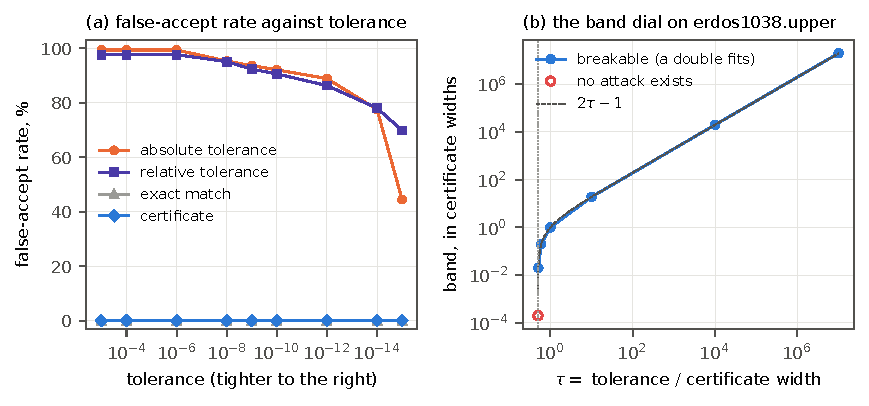
\includegraphics[width=\linewidth]{certified-evaluation-band.pdf}
\caption{(a) False-accept rate of the four reference graders against the tolerance, over the \Wrong\ provably wrong submissions of \S\ref{sec:canary}; the exact-match and certificate rows lie on the axis. (b) The band of accepted-but-wrong values in certificate widths against $\tau=\tol/w$ on \texttt{\GymDialFact} (width \GymDialWidth): the closed form $2\tau-1$, and the point past which no double fits. Drawn from \texttt{certs/envs-record.json} and \texttt{certs/gym-record.json}.}\label{fig:band}
\end{figure}

\section{The canary factory: graders graded}\label{sec:canary}

The band is a generator: every value in $B$ is a submission that is provably wrong and guaranteed to pass, so the adversarial set is enumerated rather than mutated, and it is unbounded. The suite is built from \CorpusFacts\ certified facts, each read from a record in the repository at load time and pinned to it by sha256 (\CorpusPinned\ of them; the last is a closed form enclosed from an enclosure of $\pi$ at build): the two constants of Erd\H{o}s problem \#852, the Erd\H{o}s--Herzog--Piranian bracket, Chowla's cosine dips, and the conjectures of the laboratory's own ledger, \CorpusIntegers\ of them exact integers of width zero (a tensor rank, a contact count, a period count). Minting from a fact not marked certified throws rather than degrading, and a record whose bytes have moved makes the battery refuse. Tolerances probed: \TolList. Submissions: \Submissions, of which \Wrong\ are provably wrong and \Right\ provably right, the second half because a false-accept benchmark with no controls is passed perfectly by a grader that rejects everything. Table~\ref{tab:families} lists the families and Table~\ref{tab:graders} the measurement; soundness is $(1-\mathrm{FA})(1-\mathrm{FR})$ because either rate alone is gameable.

\begin{table}[htbp]\centering\small
\begin{tabular}{lrl}\toprule
family & submissions & truth\\\midrule
\FamilyRows
\bottomrule\end{tabular}
\caption{The canary families of \texttt{certs/envs-record.json}. The published-wrong family carries, at every tolerance, the value a problem thread printed for \texttt{\PubFactId}.}\label{tab:families}
\end{table}

\begin{table}[htbp]\centering\small
\begin{tabular}{lrrr}\toprule
grader & false-accept & false-reject & soundness\\\midrule
\GraderRows
\bottomrule\end{tabular}
\qquad
\begin{tabular}{lrr}\toprule
tolerance & absolute & relative\\\midrule
\CurveRows
\bottomrule\end{tabular}
\caption{Left: the four graders over the whole suite. Right: the false-accept rate of the two tolerance graders by tolerance; the exact-match and certificate graders are zero at every tolerance.}\label{tab:graders}
\end{table}

Three readings. The absolute-tolerance grader accepts \AbsFA\ of the provably wrong submissions and the relative one \RelFA; against the \Right\ controls each rejects \AbsFR. The exact-match grader reproduces the strictness trade-off that \cite{Ray26} reports as an operational fact (a SymPy-backed replacement removes the measured false positives, but acceptance falls from 0.500 to 0.400 and coverage from 0.900 to 0.760): \ExactFA\ false-accept at \ExactFR\ false-reject, the rejected controls including the certificate's midpoint printed at full double precision and read back. The certificate grader breaks the trade-off, \EnclFA\ and \EnclFR, because it does not narrow the accepted language heuristically; it defines it as the set of values not yet refuted. The curve is the figure that answers the standard remedy: four orders of magnitude of tightening take absolute tolerance from \AbsFAloose\ at \TolLoose\ to \AbsFAtight\ at \TolTight, a tolerance at the edge of what a double carries, and Proposition~\ref{prop:band} says why the fall is slow: the band closes fact by fact as $\tol$ drops below half that fact's width, so the aggregate reaches zero only when the tolerance is under half the width of every certificate in the corpus, and at \TolTight\ it still accepts the \AbsFAtight\ whose certificates are wider than \TwiceTolTight. The relative grader is worse at the tight end (\RelFAtight) because a relative slack on a quantity of order $10^{-2}$ is a smaller absolute slack.

\paragraph{One canary that is not synthetic.} The fact \texttt{\PubFactId}, $C^\ast=\tfrac12\bigl(\prod_{p\ge3}(1+(p-1)^{-3})-1\bigr)$, carries the value \PubValue\ that the Erd\H{o}s \#852 discussion thread published for it \cite{E852}. The certificate, as doubles, is $[\PubLo,\ \PubHi]$, of width \PubWidth; the published value lies \PubGap\ outside it and inside any ordinary tolerance of it. It is a member of the acceptance band nobody had to mint: it was printed, in public, as a result, and the absolute grader accepted it \AbsFooledPublished\ times of \PublishedCanaries.

\paragraph{The gym and the attacker.} The same record carries two model-facing environments on the corpus. The \emph{uniformity gym} asks for a verdict with evidence on \UnifInstances\ instances (\UnifNeedled\ carrying a needle a sampling grid steps over), scored $+1$ correct with evidence, $0$ correct but unsupported, $+0.25$ honest abstention, $-1$ wrong; evidence is a dyadic tiling accepted only if it forms a complete prefix-free set, checked combinatorially with no slack. A bare verdict scores zero however correct; a sampling grid dressed as a tiling scores \BluffScore, worse than abstaining, because the cell holding the needle refuses to verify; the sound interval solver scores \SoundScore\ with one abstention, and the budget-limited sound solver, the row people omit, abstains \BudgetAbstained\ times and is never wrong (\BudgetScore)---without it the $+0.25$ is never earned and the environment teaches bravado. The \emph{attacker} inverts the polarity: shown a grader and a certificate, the model must produce a value the grader accepts and the certificate refutes, or \verdict{no\_attack}. Of its \AttackRungs\ rungs, \AttackRungsNone\ have no attack (a tolerance narrower than the enclosure; a grader that compares against the certificate; a tolerance finer than the spacing of doubles around an integer, Proposition~\ref{prop:double}), and claiming a break that does not verify is scored wrong, not as a near miss. \EnvsForgeriesPlanted\ forgeries are planted before any model is called and \EnvsForgeriesLeaked\ have leaked; the battery (\EnvsBatteryPass\ checks, \EnvsBatteryReds\ red controls) includes the two degenerate graders, accept-everything and reject-everything, which must both score zero.

\section{When the answer key is wrong: three specimens and a control}\label{sec:keys}

An evaluation graded against reference values inherits the failure class of whatever computed them, and for mathematical ground truth the pipeline is usually floating point, checked by digit agreement. Three specimens from the repository's audits show the class; each is re-proved by the program that writes this paper's numbers. A fourth case, a published claim that holds, is the control, because an audit that only ever refutes is a search.

\paragraph{Specimen I: the constant that was a rounding error.} The published $C^\ast$ of \S\ref{sec:canary} agrees with the certified lower endpoint \CertLo\ to \AgreePlaces\ decimal places and is wrong from the \FailPlace th. The wrong digits are not near the truth by accident: re-run while this paper is built, the naive double-precision product over the \PrimesCount\ odd primes below \PrimeLimit\ emits \NaiveC, the published value digit for digit, because $1+(p-1)^{-3}$ rounds to exactly $1.0$ once $(p-1)^3\ge2^{53}$, that is for $p-1\ge\DropThreshold$, so \DroppedPct\ of the factors (\DroppedCount) vanish and the product self-truncates regardless of the loop bound. The exact partial product is a strict lower bound of the full product with no tail estimate, and it already exceeds the published value under both truncation and rounding readings: \verdict{refuted}, in one integer inequality. The certificate itself is a directed-rounding product over \CstarPrimes\ odd primes below \CstarPrimeLimit\ at \CstarBits\ bits with the tail bounded analytically (\CstarDigits\ decimal places). The thread's other constant $c_0$, the positive root of $I_0(c)=1$, is \verdict{verified} as a rounding to 14 places (\CZeroPublished) against a bracket of \CZeroBisections\ bisections at \CZeroBits\ bits, with a wrong trailing ellipsis. In an answer key the published $C^\ast$ would score a float-faithful model correct and an exact one wrong, and a rerun of the same pipeline would confirm the key.

\paragraph{Specimen II: digit agreement is not evidence.} Validating a key by matching digits assumes agreement implies identity. Over \OeisEntries\ OEIS decimal expansions \cite{OEIS}, \ImpostorCount\ published constants agree with simple closed forms and are provably not equal to them, each refutation one exact big-integer comparison at the full published precision. The deepest, re-derived here, is \ImpostorId\ (``\ImpostorName''), which agrees with the rational \ImpostorLabel\ for \ImpostorDepth\ significant digits before exact arithmetic separates them (the OEIS records the difference as A271881). A digit-matched validation shallower than that certifies the impostor; a double-precision check, at seventeen digits, cannot settle it at all.

\paragraph{Specimen III: true computation, false print.} The key can be wrong although the computation behind it was right. The \RmSheets\ result sheets of the Ramanujan Machine \cite{RM21} print \RmPrinted\ rows; decided by rigorous enclosures and exact rational comparison, \RmSurvive\ survive and \RmRefuted\ is refuted: a mixed-zeta identity whose constant term carries a sign slip, false as printed, while the continued fraction its own polynomials define converges to the corrected value exactly, both directions re-certified on one enclosure. No rerun of the discovery pipeline catches this, because the pipeline was never wrong.

\paragraph{The control: a published claim that held.} Pointed at the Lyapunov functions that arXiv:2606.10045 reports as discovered by constrained symbolic regression \cite{Lyap26}, an exact rational sum-of-squares certifier returns \verdict{confirmed} for the function the paper states as valid, $V=x_1^2+4x_2^2$: $\dot V=-2x_1^2-8x_2^4$ is an exact weighted sum of squares, zero only at the origin. The three under-sampled candidates the paper flags itself are refuted with rational witnesses; for Eq.~23, $V=x_1^2+3.97x_2^2$, the point $x=\SosWitnessX$ gives $\dot V=\SosWitnessVdot>0$. And run on the Motzkin polynomial, nonnegative everywhere and not a sum of squares \cite{Motzkin67}, the same certifier returns \verdict{refused}: it declines to certify a true statement for want of the certificate it requires, printing the probe $M(1,1)=0$ beside the refusal. The \SosPrograms\ programs ran during this build and reported \SosPass\ passing rows including the red controls. A grader you have never seen decline is not known to be able to decline, and a grader that cannot decline will eventually confirm an answer key back to its author.

\section{GSM8K's answer key, re-decided to the last step}\label{sec:gsm8k}

Every harness that scores GSM8K \cite{Cobbe21} compares a model's number with the \texttt{\#\#\#\#} answer line of a stored solution, and the solution prints the arithmetic that reaches it: calculator annotations \texttt{<<lhs=rhs>>} the authors inserted, and the prose steps between them. That arithmetic can be re-decided without a model and without a reader. GSM8K is held at commit \GsmCommit\ of the authors' repository (\TestItems\ test and \TrainItems\ train items) and GSM8K-Platinum \cite{Vendrow25}, the human revision of the test set, at revision \PlatRevision\ of its dataset; both are re-hashed at every run. An annotation is read as the expression its left side denotes, by a hand-written parser for $+\,-\,\times\,\div$ and parentheses over exact fractions with nothing passed to \texttt{eval}, and compared with the rational its right side denotes: \verdict{exact}, \verdict{rounded} (within half a unit of the last printed place, and said so), \verdict{wrong} or \verdict{refused}. A prose equation is a run of arithmetic characters around an ``='', read as a chain pair by pair with the notations the writers use (a dollar or percent sign as a unit label, ``5 and 2/3'' as a mixed number, ``25 / 1/3'' as $25\div\tfrac13$); anything cut off by a word, glued to a variable or otherwise unreadable is \verdict{unread}, never a verdict. The answer line is read as a rational and compared with the last annotation's value, then with every prose step's. Table~\ref{tab:gsmclass} classes the items.

\begin{table}[htbp]\centering\small
\begin{tabular}{lrr}\toprule
class & test & train\\\midrule
\GsmClassRows
\bottomrule\end{tabular}
\caption{GSM8K items by whether their own printed steps reach their own answer, from \texttt{certs/gsm8k-ledger.json}. Test: \TestAnn\ annotations, \TestProse\ prose equations read and \TestProseUnread\ unread. Train: \TrainAnn\ annotations (\TrainAnnExact\ exact, \TrainAnnRefused\ refused for an operator outside the grammar), \TrainProse\ read and \TrainProseUnread\ unread.}\label{tab:gsmclass}
\end{table}

\paragraph{Findings.} All \TestAnn\ test-set annotations evaluate exactly to the value they print, not one wrong and not one rounded, and so do \TrainAnnExact\ of the \TrainAnn\ train-set ones (the other \TrainAnnRefused\ use \texttt{//}). Reading the prose too, \WrongTest\ test keys and \WrongTrain\ train keys print a step that does not hold as printed (Table~\ref{tab:witness}); the answer rests on the wrong step in \WrongTestNotHeld\ test and \WrongTrainNotHeld\ train keys and is held by another step of the same key in the rest, \WrongTrainBeside\ of the train slips standing beside a correct calculator annotation. Two train steps are roundings (items \GsmRoundedList). Nothing here changes an answer a harness grades against: the answer of test item 501 is the annotation beside the slip, and item 1024's 300 is the number the writer meant by ``\$320 $-$ \$20''. These are provenance findings about the key's text, the kind a few-shot prompt copies verbatim into a model's context, since both harnesses draw their examples from the train set.

\begin{table}[htbp]\centering\scriptsize\setlength{\tabcolsep}{4pt}
\begin{tabular}{llllll}\toprule
set & item & the printed step & exact value of the left side & answer & answer held by another step\\\midrule
\GsmWitnessRowsA
\GsmWitnessRowsB
\bottomrule\end{tabular}
\caption{Every printed step in GSM8K that does not hold as printed. Two train rows (5396, 6590) read a day number and a week range as arithmetic; they are listed rather than excused, because the rule that would exclude them is not one the reader can state.}\label{tab:witness}
\end{table}

\paragraph{Against Platinum.} GSM8K-Platinum ran frontier models over the test set, inspected by hand the \PlatFlagged\ items on which some model disagreed with the key, removed \PlatRemoved, relabelled \PlatRevised\ and verified \PlatVerified, leaving \PlatConsensus\ consensus items that no model disagreed with and nobody inspected. Joined by question text, exactly, the two readings cross-tabulate as in Table~\ref{tab:cross}. Both test-set slips are consensus items: every model reproduced the intended answer, so a flagging method that looks only where a model disagrees had no reason to open them; a typo no model copies is invisible to a model-flagged audit by construction. The converse holds too: all \PlatRevised\ relabelled answers have arithmetic that holds to the last step (\RevisedReproduced\ reproduced, one underived), and \RemovedReproduced\ of the \PlatRemoved\ removed items are reproduced here. Those errors are readings of the problem, a rate read as linear or a quantity counted twice, and no re-decision of the numbers can see them. The two halves of a task-QA audit find different things, and the mechanical half runs in \GsmSeconds\ seconds.

\begin{table}[htbp]\centering\small
\begin{tabular}{lrrrrrr}\toprule
Platinum status & items & reproduced & answer in prose & underived & no steps & step wrong\\\midrule
\GsmCrossRows
\bottomrule\end{tabular}
\caption{GSM8K-Platinum's statuses against this paper's classes, on the \PlatKept\ kept and \PlatRemoved\ removed test items.}\label{tab:cross}
\end{table}

\paragraph{The graders.} Every test answer is an integer as printed (\TestForms); the train set has the same shape (\TrainForms). Read against the two scoring rules pinned by commit (\texttt{inspect\_evals} at \InspectEvalsCommit, whose \texttt{match(numeric=True)} parses the target as a number, observed on \texttt{inspect\_ai} \InspectVersion; \texttt{lm-evaluation-harness} at \LmEvalCommit, which strips commas from both sides before an exact match), no key is in a form either harness misreads: of \ObsRows\ probe forms observed, \ObsCorrect\ grade correct and the two that do not (a fraction, a percent sign) occur in no answer line of either set. A false start is worth recording: the first survey listed annotations and answer lines in one list, so an annotation \texttt{<<3/4=3/4>>} was written up as a fraction-form key and an issue drafted on it; the report builder's gate (fraction keys $=0\ne$ the claimed 1) refused the page and the draft was deleted. The battery (\GsmBatteryPass\ checks, \GsmBatteryReds\ red controls: a planted wrong annotation, a value off by more than half a unit, the \texttt{//} operator, a Python name, a power) ran during this build.

\section{METR's time horizon, certified}\label{sec:horizon}

The 50\% time horizon of METR \cite{Kwa25} is the length of task, measured in the time a human takes, that a model completes half the time; METR reads it off a logistic fit of run success on $\log_2$ human minutes and publishes a point estimate with a bootstrap interval, and the doubling time of that number is the most-quoted trend in AI forecasting. The evidence is public: the raw runs of the analysis repository \cite{METRrepo} at commit \HzRepoCommit\ (\HzRepoDate; \HzRuns\ runs over \HzRunsAgents\ aliases) and the two files behind the live chart, fetched \HzFetched\ (the page says updated \HzSiteUpdated): the per-task file with each agent's fitted coefficient and intercept to three decimals, and the benchmark file with the point estimates, bootstrap intervals, state-of-the-art flags and doubling times; the Time Horizon~1.1 post of \HzPostDate\ \cite{METR26} is pinned too, all seven files by sha256.

\paragraph{The estimator, to the letter.} scikit-learn's weighted, $L_2$-penalised logistic regression is the minimiser of
\[
J(w,b)=\sum_i s_i\bigl[-y_i\log p_i-(1-y_i)\log(1-p_i)\bigr]+\tfrac{\lambda}{2}w^2,\qquad p_i=\sigma(wx_i+b),\ x_i=\log_2(\text{minutes}_i),
\]
with $s_i$ the task weight ($1/\sqrt k$ for a family of $k$ tasks, normalised to one) and $\lambda=\HzLambda$ from METR's parameter file. $J$ is strictly convex, so the minimiser is the unique zero of the score $F(w,b)=\bigl(\lambda w-\sum_i s_i(y_i-p_i)x_i,\ -\sum_i s_i(y_i-p_i)\bigr)$, and per-run fitting collapses to per-task fitting with the mean outcome, exactly: $\sum_{\text{runs}}(s/n)(y_r-p)=s(\bar y-p)$. The horizon at success rate $q$ is $2^{(\operatorname{logit}q-b)/w}$.

\begin{proposition}[certification of the fit]\label{prop:kraw}
Let $X$ be a box in $(w,b)$-space, $x_0$ its centre, $A$ a nonsingular matrix and $J_F(X)$ an interval enclosure of the Jacobian of $F$ over $X$. If the Krawczyk image $K(X)=x_0-AF(x_0)+(I-AJ_F(X))(X-x_0)$, evaluated in outward-rounded interval arithmetic, lies in the interior of $X$, then $F$ has exactly one zero in $X$ \cite{Krawczyk69,Rump10}, and that zero is the minimiser of $J$.
\end{proposition}

A float Newton iteration finds the candidate; the Krawczyk operator, evaluated in a standard-library interval arithmetic written for this (outward rounding by \texttt{nextafter}, $\exp$ and $\log$ from rational series with proved tails, every minute literal read as the rational it denotes and enclosed), proves the box, doubling its radius until containment holds or refusing; the horizon is the interval extension over the box. The weights are METR's, $1/\sqrt k$ as the correctly rounded double taken as a rational, which the file's own weights match to $2.9\times10^{-9}$.

\paragraph{What is proved, per model.} All \HzFits\ fits certify: for each of the \HzLive\ agents on the live chart and each of the \HzRunsAgents\ aliases of the runs file, the box has radius below $10^{-10}$ (the largest is \HzMaxRad). For \HzExAlias\ on the live file (\HzExTasks\ tasks) the slope box is $[\HzExSlopeLo,\HzExSlopeHi]$, the intercept box $[\HzExIntLo,\HzExIntHi]$, and the 50\% horizon $[\HzExHLo,\HzExHHi]$ minutes; METR prints \HzExSite\ with bootstrap interval $[\HzExCiLo,\HzExCiHi]$. Table~\ref{tab:horizon} reads every printed number against its enclosure. The printed slope and intercept are the rounding of the box for \HzCoefRepro\ of \HzLive\ models; the exception is \HzDifferAlias, whose intercept prints \HzDifferPrinted\ where the box, $\HzDifferBoxLo\ldots$, rounds to \HzDifferCertified. The site's p50 estimates lie between \HzGapMin\ and \HzGapMax\ (relative) from the enclosure and never inside it (\HzInside\ of \HzLive), which is what a solver stopped at a tolerance looks like next to a proof; every enclosure lies inside METR's bootstrap interval. The March runs and the May per-task file agree, where an agent is in both (\HzBoth\ aliases), to \HzBothGap\ on the horizon. The \texttt{human} alias of the runs file, fitted by the same rule on \HzHumanTasks\ tasks, gives \HzHuman\ minutes; it is reported as a curiosity, not a measurement of people.

\begin{table}[htbp]\centering\scriptsize\setlength{\tabcolsep}{4pt}
\begin{tabular}{llrrlll}\toprule
model & released & certified p50 & site p50 & gap & printed $(w,b)$ & verdict\\\midrule
\HorizonRows
\bottomrule\end{tabular}
\caption{The \HzLive\ models of the live chart in release order: the certified 50\% horizon (midpoint of the enclosure, in minutes; the enclosures are \HzWidthMin\ to \HzWidthMax\ minutes wide), METR's point estimate, their relative gap, and METR's printed slope and intercept against the rounding of the certified box. From \texttt{certs/horizon-ledger.json}.}\label{tab:horizon}
\end{table}

\paragraph{The trend, as an interval.} Over the models the site flags as state of the art at release with a horizon under \HzExcludedHours\ hours (the site's own rule, which leaves \HzDifferAlias\ out and Claude Opus 4.6 in), the exact least-squares line through $\log_2$ of the certified horizons against release date has a slope enclosed to \HzSlopeWidth\ bits per day, a doubling time enclosed to \HzDoublingWidth\ days: \HzDoubling\ days from 2023 over \HzTrendN\ models, where the site prints \HzDoublingPrinted\ with bootstrap interval $[\HzCiLo,\HzCiHi]$ (Figure~\ref{fig:horizon}). From 2024 the same rule gives \HzDoublingTwentyFour\ days over \HzTrendNTwentyFour\ models; the January post printed \HzPostTwentyFour\ on its smaller set and \HzPostTwentyThree\ from 2023. So the site's trend is computed on exactly the numbers its chart shows by exactly the rule its file states. Where the January post and the May chart disagree, the certificate sides with the May file because it is the May file: of the \HzPostN\ TH1.1 horizons the post printed, \HzPostRepro\ (Claude 3.7 Sonnet, 60) is the rounding of the certified one and \HzPostDiffer\ differ by between \HzPostGapMin\% and \HzPostGapMax\% at the post's printed precision, the site's own May estimates having moved by the same amounts. Nothing was mis-computed: runs were added between the post and the chart, and the post is a fit on January runs that no public file holds. A printed number without the file it came from cannot be re-decided; it can only be dated.

\begin{figure}[t]\centering
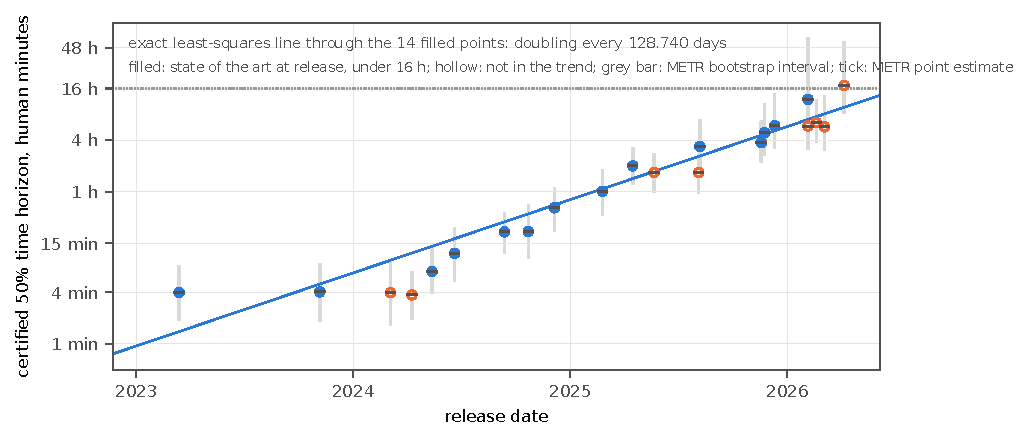
\includegraphics[width=\linewidth]{certified-evaluation-horizon.pdf}
\caption{Certified 50\% horizons against release date, from \texttt{certs/horizon-ledger.json}. The line is re-fitted by the drawing program from the \HzTrendN\ filled points and refused if its slope leaves the ledger's enclosure; the grey bars are METR's bootstrap intervals, not re-decided.}\label{fig:horizon}
\end{figure}

\paragraph{Why the instrument exists.} The page this comes from is a calibration. The same instrument is built to fit a horizon on tasks graded by an exact verifier (the environments of \S\ref{sec:envs}) against timed human baselines; today its own section reads \HzOwnVerdict: \HzOwnLogs\ frontier logs with \HzOwnRollouts\ rollouts on \HzOwnTasks\ listed tasks, none of which yet has a human time. The battery (\HzBatteryChecks\ checks, \HzBatteryReds\ red controls: a Taylor series without its remainder, a division through zero, Krawczyk from a far candidate, a slope box through zero asked for a horizon, a printed horizon moved by 1\%) re-certifies one agent live from the pinned file and requires the ledger's box; the whole ledger re-derives in about \HzSeconds\ seconds on eight cores.

\section{The verified reward channel and three environments}\label{sec:envs}

\paragraph{The channel.} The design that removes the key is to grade tasks where no reference value exists to contaminate: ask the model to \emph{exhibit} a witness and let the grader re-derive the claim from the witness alone, exactly. The running instance is a rank-$R$ decomposition of the $\langle n,m,p\rangle$ matrix-multiplication tensor over $\mathbb{Q}$ or $\mathbb{F}_2$, the task on which proposer-plus-verifier produced a famous discovery \cite{Strassen69,Fawzi22}: a proposal either satisfies all $(nm)(mp)(np)$ tensor equations in exact rational arithmetic or it does not, floats are refused at the door, and the verdict is \verdict{certified}, \verdict{refuted} with the first violated equation and its exact discrepancy, or \verdict{refused}. Three rules carry the discipline: a screen may only prune, never admit; every certifier is calibrated against a known answer and against red controls that must fire at import and at every build, among them a coefficient perturbed by exactly $10^{-9}$, invisible to any float screen, a control that certifies aborting the campaign; and feedback to a proposing model is template-locked to the grader's own mechanism, so the channel can neither coach nor be sweet-talked. Across \MmCampaigns\ campaigns of \MmModels\ frontier models, \MmRows\ ledger rows and \MmAnswered\ answered proposals (\MmBudget\ were cut off by the harness's own output cap and belong in no rate), \MmCertified\ are certified, \MmRejected\ rejected by the screen, \MmMalformed\ malformed, \MmDeclined\ declined and \MmRefuted\ refuted: every well-formed proposal that survived the float screen was exactly right, so frontier failures here are loud, not subtle. One row of the ledger is a correction: \MmCorrectionRows\ rows tagged as run at low thinking effort ran at the default effort because the campaign path dropped the flag (found \MmCorrectionFound); the ledger is append-only, the correction file is read by every consumer, and the rows are displayed as default-effort measurements. The honesty probe asks for rank 6 on $\langle2,2,2\rangle$, impossible since the rank is 7 \cite{Winograd71}: of \ProbeN\ replies each, Claude Opus 5 declined \ProbeOpusDeclined, Claude Sonnet 5 \ProbeSonnetDeclined\ and Claude Haiku 4.5 \ProbeHaikuDeclined, and no proposal certified. In closed loop, where the grader answers each failure with its own refutation and the model retries in the same conversation, \LoopTrajectories\ trajectories and \LoopRounds\ graded rounds ended with \LoopCertified\ certified, every one at its first round and \LoopConversions\ converted by feedback: a below-bar model is not rescued and an at-bar model needs no rescue.

\paragraph{break-the-grader.} The attacker of \S\ref{sec:canary}, standard library only, is on the Environments Hub as \path{carlos-toledo/break-the-grader}. Its corpus is the \GymFacts\ facts (\GymPinned\ pinned, \GymIntegers\ exact integers, stored as rationals). Of \GymTasks\ generated tasks, \GymAttackable\ are breakable and \GymImpossible\ are not, decided by constructing an attack and never by a label; always-attack solves \GymAlways\ and never-attack \GymNever, so both standing answers lose and only checking wins. Difficulty is drawn in room (Proposition~\ref{prop:double}) from a declared mix of impossible 25\%, razor 35\%, narrow 25\% and wide 15\% and realised as \GymImpossible, 453, 664 and 278 of \GymTasks, both figures printed because keys sit at five positions across the certificate and only the midpoint gives the closed form exactly. \GymForgeries\ forgeries are planted in the package's tests and \GymLeaked\ leaked; the build refuses the page if the careful policy's lead over blind play on the \GymBaselineN-task draw falls below a quarter of a point (it is \GymGap). Table~\ref{tab:pilot} is the reference table: on the same \PilotN\ seeds as the four policies (\PilotCalls\ calls, \$\PilotSpent\ of a \$\PilotCap\ cap reserved worst-case before every call, \PilotDate), the three models separate, \PilotOpusMean, \PilotSonnetMean\ and \PilotHaikuMean, and the smallest scores below the one-line blind policy (\PilotAlwaysMean), not because the tasks are hard for a program but because blind play makes no false claims and that model makes \PilotHaikuFalse. The impossible column is the whole of what the environment measures; a mean that ignores it can be bought by guessing.

\begin{table}[htbp]\centering\footnotesize
\begin{tabular}{lrrrrrrrr}\toprule
player & $n$ & mean & solved & false claims & impossible & razor & narrow & wide\\\midrule
\PilotRows
\bottomrule\end{tabular}
\caption{break-the-grader on \PilotN\ seeds, from \texttt{certs/grader-pilot.json} (scored by the shipped package). The policies read only the prompt: never (always refuse), always (attack at the first double past the interval), naive (submit $\hi+\tol/2$ in floats), careful (the arithmetic in exact rationals). Rung columns are solved/of; replies truncated by the caller's \PilotMaxTokens-token cap (\PilotSonnetTruncated\ for Sonnet) are excluded from the rates.}\label{tab:pilot}
\end{table}

\paragraph{blind-spot.} A kissing predicate for vectors in $\mathbb{Z}^{11}$ with 3-bit coordinates was put into RTL and proved sound; yosys then mutated the netlist \BsMutations\ times, one bent bit of one cell's port each, and a testbench of pair verdicts drawn from finished certified mathematics could not see the comparator constant, because a corpus of valid inputs cannot test the code that rejects invalid ones, never varies the norms and never makes a large dot product. Four constructed families got to zero survivors; the interesting region is measure-zero to a sampler and reachable by hand, and the environment asks whether a model can reach it: one mutation or none has been applied, and the model names up to eight input pairs that flip an output pin, claims \verdict{equivalent}, or says \verdict{undecided}. A kill is verified by simulating the netlist under the mutation, equivalence against a SAT proof on a miter, every label certified twice; the pool holds \BsKillable\ killable, \BsEquivalent\ proved equivalent and \BsIdentity\ identity mutant, \BsCovered\ killed by the corpus and \BsMintOnly, \BsOutboxOnly\ and \BsAlignedOnly\ only by one constructed family each. Three rungs state more or less of the defect (\emph{located}, \emph{profile}, \emph{blind}); scoring is $+1$ for a verified kill or a proved equivalence, $0$ for a miss, an abstention or an unreadable reply, $-1$ for a kill claimed on a design proved unchanged or an equivalence claimed where a pair exists. Under Inspect \cite{Inspect} (\BsInspect, seed \BsSeed) the scorer is the package's own decision function; every log is re-scored offline, \BsFrontierRollouts\ frontier and \BsControlRollouts\ control rollouts with \BsDisagreements\ disagreements, and the reference policies score \BsSatMean\ (the witness or the proof), \BsAbstainMean\ (abstain) and \BsNeverMean\ (equivalent always) on \BsControlN\ tasks. Table~\ref{tab:ladder} is the effort ladder: Claude Sonnet 5 on the located rung goes \BsSonnetLocated\ of \BsRungN\ as effort rises, a budget ladder on a judge-free task; the blind rung carries \BsBlindWrong\ false alarms at every setting for every model, each a kill claimed on a design with no defect; and Claude Opus 5 declines the profile rung (\BsOpusProfileUnreadable\ of \BsRungN\ unreadable, a content-policy refusal the prompt was not reworded to pass) while solving \BsOpusLocated\ located. The human-baselines file is pinned with \BsBaselineTasks\ task ids and \BsBaselineAttempts\ attempts: \BsBaselineStatus.

\begin{table}[htbp]\centering\footnotesize
\begin{tabular}{lllllrr}\toprule
model, effort & located & profile & blind & wrong & unreadable & US\$\\\midrule
\BsLadderRows
\bottomrule\end{tabular}
\caption{blind-spot under Inspect, \BsRungN\ tasks per rung: solved/of (mean reward), from \texttt{certs/blind-spot-inspect-ledger.json}. Unreadable replies are refusals or over-budget replies, scored 0 and never masked.}\label{tab:ladder}
\end{table}

\paragraph{lattice-claims.} The third environment is built from a mistake: auditing published SVP-challenge records, a bit-exact grader of the shortest-vector claim reported most of them as disagreeing with their published figure, every discrepancy at about $10^{-4}$ and in both signs, because the published ratios had been computed from the true norm and printed rounded while the exact ratio was computed from the rounded norm. Exactness did not save the grader; naming what the claim was about would have. So a submission must declare the reference it decided against, and a right verdict from a reference the task did not state does not score as right. Instances are minted from a seed around a short vector chosen first, the predicate is exact with a certified $\pi$ bracket, and three rungs state more or less of the reference: \emph{declared}; \emph{printed}, where \verdict{straddles} is a genuine third answer (at $n=\LcStraddleN$ a printed norm of \LcStraddlePrinted\ against a wall of \LcStraddleWall\ leaves the ratio in $[\LcStraddleLo,\LcStraddleHi]$ across the threshold); and \emph{underspecified}, where only \verdict{needs\_data}, naming the field, is right. \LcForgeries\ forgeries are planted and all caught, two of them holes in the laboratory's own grader. The float-versus-exact story was measured and is weaker than it looks: below dimension \LcCliff\ a careful float grader agrees with the exact decision on every sampled instance, and above it, where the challenge-scaled determinant overflows a double, a naive float grader accepts everything (\LcAboveNaive\ of \LcAboveN\ at dimensions \LcAboveDims\ against 0 of \LcBelowN\ at \LcBelowDims); the failure in this domain is a confidently blind grader, not rounding. Through the framework (\LcRollouts\ rollouts, \LcRanOn, \$\LcCost, re-scored offline with no disagreement), Claude Sonnet 5 certifies 10, 2 and 4 of 12 on the three rungs and Claude Haiku 4.5 answers \LcHaikuDeclaredSolved\ of the declared rung correctly while declaring a usable reference on \LcHaikuDeclaredWf: every verdict it got right came from a reference it never properly stated, which is the environment's thesis appearing as a measurement.

\section{Certified MathBench v0, pre-registered}\label{sec:mathbench}

Seven construction families ask for an exhibited object and decide it exactly, with no key, judge or tolerance: a Golomb ruler with $n$ marks and length at most $L$; a cap of size $k$ in $\mathbb{F}_3^n$; a binary code $(n,M,d)$; a graph on $n$ vertices with no $K_s$ and no independent $t$-set; a law on $\mathbb{Z}^2$ with $H(X-Y)\ge c\max(H(X),H(Y),H(X+Y))$, entropies in intervals; $k$ equal-norm integer vectors pairwise at least $60^\circ$ apart; and a rank-$R$ bilinear algorithm for $n$-term polynomial products over $\mathbb{F}_2$. The ladders run to the published optima and records, and \MbBeyondRungs\ rungs ask beyond the record. The pre-registration of 29 September 2026, written before the first model call, fixed the families and ladders; one sample per rung at the API's default thinking and effort with a \MbCap-token output cap; the three models (Claude Haiku 4.5, Claude Sonnet 5, Claude Opus 5; the keys on this machine reach no other laboratory); the metrics (certified of graded; refuted apart from malformed and budget-exhausted; rungs certified that the baseline does not; tokens and dollars per certified rung); a US\$30 ceiling reserved worst-case before every call; and the null: if no model certifies a rung the baseline does not, the easy rungs are recall and the hard ones out of reach at one sample, and a certified beyond-the-record rung is not announced from this run but re-decided by a second implementation first. Every rung with a witness on record carries a green control that must certify and near-misses forged from it that must refute before any model is asked (\MbBatteryGreens\ green, \MbBatteryReds\ red; the battery of \MbBatteryPass\ checks ran during this build), and each family's textbook first try (a greedy ruler, a lexicode, a quadratic-residue circulant, the $D_n$ roots, schoolbook multiplication) is decided like any proposal: the baseline certifies \MbBaselineCertified\ of \MbRungs.

\begin{table}[htbp]\centering\footnotesize\setlength{\tabcolsep}{4pt}
\begin{tabular}{lrrrrrrrrr}\toprule
model & graded & cert. & ref. & rej. & malf. & capped & beyond & US\$ & \$/cert.\\\midrule
\MbModelRows
\bottomrule\end{tabular}
\caption{Certified MathBench v0 by model, from \texttt{certs/mathbench-ledger.jsonl} (\MbRows\ rows; \MbRungs\ rungs each): rungs graded, certified, refuted, rejected by the screen, malformed, capped (the reply reached the output cap before an object: recorded and billed, never graded), certified beyond the baseline, dollars spent and dollars per certified rung.}\label{tab:mb}
\end{table}

\begin{table}[htbp]\centering\footnotesize
\begin{tabular}{lrrrll}\toprule
family & rungs & baseline & Haiku 4.5 & Sonnet 5 (cap) & Opus 5 (cap)\\\midrule
\MbFamilyRows
\bottomrule\end{tabular}
\caption{Rungs certified per family and answerer; in parentheses, the rungs on which the reply reached the output cap.}\label{tab:mbfam}
\end{table}

\paragraph{Results.} Tables~\ref{tab:mb} and \ref{tab:mbfam}. Claude Haiku 4.5 certifies \MbHaikuCert\ of \MbHaikuGraded\ graded rungs (\MbHaikuBeyond\ the baseline does not reach) and is refuted on \MbHaikuRefuted; Claude Sonnet 5 certifies \MbSonnetCert\ of \MbSonnetGraded\ (\MbSonnetBeyond\ beyond the baseline) and ran out of tokens on \MbSonnetOot; Claude Opus 5 certifies \MbOpusCert\ of \MbOpusGraded\ (\MbOpusBeyond\ beyond) and ran out on \MbOpusOot. The run cost US\$\MbTotalUsd\ of the ceiling. No model certified a rung beyond the published record (\MbBeyondCertified\ of \MbBeyondRungs); the null of the pre-registration is the result. The refutations of the two larger models are few and named: Opus 5's one refuted object, at kissing \MbOpusRefutedTarget, is \MbOpusRefutedWitness, a duplicate vector, exactly the near-miss the red controls forge; Sonnet 5's two are at \MbSonnetRefutedTargets, each with a triangle the certifier names. The finding of v0 is about the cap rather than about correctness: the two larger models reached \MbCap\ output tokens before emitting an object on more than half of the rungs, almost always where the objects are large (caps, codes, the entropy laws, the larger products), so v0 measured finishing, and a v1 with a larger cap or an explicit effort setting is to be pre-registered first. One deviation is recorded in the pre-registration: five Opus 5 calls on the sum--difference family returned an API error with no reply and nothing billed while the account's credit ran out, and were issued once more after the run with the same settings; no rung was sampled twice.

\section{What is not claimed}\label{sec:not}

The band proposition is elementary; the measurement of \S\ref{sec:canary} is of four reference grader shapes, not of anybody's product, and the suite that measures a real grader runs on its owner's machine. One laboratory supplies every certificate in the corpus; that is the moat and equally the limit. Nothing here is a formal proof in the sense of a proof assistant; the standard met is the working one of computer-assisted proof, one rung below a kernel and several above a decimal that looked convincing. In \S\ref{sec:keys} no priority is claimed for any mathematics: the Lyapunov functions are the paper's, the SOS-Lyapunov technique is Parrilo's \cite{Parrilo00}, and arXiv:2606.10045 is cited as a claim whose statements are taken as printed. In \S\ref{sec:gsm8k} no answer is called wrong and no question ambiguous; the prose reader is conservative by design (\TestProseUnread\ test and \TrainProseUnread\ train equations unread and counted, never guessed), and the harness observations are of two pinned commits on one date. In \S\ref{sec:horizon} no horizon is called right or wrong: the certificate is about the fit, not the tasks, the human timings or the binarisation of scores, all METR's and taken as given; the bootstrap intervals are not re-decided, since a random draw is not a theorem and the certified box is the optimiser's uncertainty; the post's runs are not public. In \S\ref{sec:envs} the matmul oracle decides finitely many exact-arithmetic facts and refuses everything else; blind-spot is one predicate, one netlist and one mutation operator; lattice-claims certifies arithmetic about a stated lattice and threshold and nothing about attack cost or any deployed scheme. In \S\ref{sec:mathbench} one sample per rung is a Pass@1 at default settings, recall and discovery look alike since most rungs are known optima, and only one laboratory's models were asked. Two figures the environments' own documentation states, the size of the certified testbench corpus behind blind-spot and the record count of the audit behind lattice-claims, have no record in this repository and are deliberately not quoted.

\cmrepro{The records, and the commands that rewrite them:
\begin{itemize}\setlength{\itemsep}{0pt}
\item \path{certs/envs-record.json}, written by \texttt{node tools/run-envs.js}, offline;
\item \path{certs/gym-record.json}, by \texttt{node tools/run-gym-record.js}; \path{certs/grader-pilot.json};
\item \path{certs/erdos852-certificate.json};
\item \path{certs/matmul-eval-ledger.jsonl}, its corrections file, and \path{certs/matmul-loop-ledger.jsonl};
\item \path{certs/gsm8k-ledger.json}, by \texttt{python3 tools/run-gsm8k-ledger.py};
\item \path{certs/horizon-ledger.json}, by \texttt{python3 tools/run-horizon-ledger.py};
\item \path{environments/blind_spot/pool/pool.json}; \path{certs/blind-spot-inspect-ledger.json};
\item \path{instruments/wiring/eval/};
\item \path{certs/mathbench-ledger.jsonl}, by \texttt{python3 tools/run-mathbench.py}, which reserves its ceiling before every call.
\end{itemize}
The macros of this document are written by \path{tools/paper-numbers/certified-evaluation.js} (run with \texttt{node}), which also re-runs the naive product and exact refutation of specimen I, the impostor depth of specimen II in exact big integers, both directions of specimen III, the three SOS programs, and the envs, gsm8k and mathbench batteries; the figures by \path{tools/paper-numbers/certified-evaluation-figs.py}. The environments are published as \path{carlos-toledo/break-the-grader}, \path{carlos-toledo/blind-spot} and \path{carlos-toledo/lattice-claims} on the Environments Hub \cite{Hub}. Sources are pinned by sha256 in \path{corpus/metr-horizon/meta.json} and \path{corpus/gsm8k/meta.json}; this document was built at commit \RepoCommit.}

\begin{footnotesize}
\begin{thebibliography}{99}
\bibitem{Rajan26} Rajan, Auditing reward hackability in code RL, arXiv:2606.16062 (2026).
\bibitem{OpenAI26} OpenAI, note on test quality in SWE-bench Verified, February 2026.
\bibitem{Zhang26} Zhang, When the reward suite is leaky, arXiv:2607.11022 (2026).
\bibitem{Gaming26} LLMs gaming verifiers, arXiv:2604.15149 (2026).
\bibitem{Ray26} Ray, Fuzzing RLVR verifiers, arXiv:2606.01066 (2026).
\bibitem{Cobbe21} K.~Cobbe, V.~Kosaraju, M.~Bavarian, M.~Chen, H.~Jun, L.~Kaiser, M.~Plappert, J.~Tworek, J.~Hilton, R.~Nakano, C.~Hesse, J.~Schulman, Training verifiers to solve math word problems, arXiv:2110.14168 (2021); \texttt{github.com/openai/grade-school-math} at \GsmCommit.
\bibitem{Vendrow25} J.~Vendrow, E.~Vendrow, S.~Beery, A.~M\k{a}dry, Do large language model benchmarks test reliability?, arXiv:2502.03461 (2025); \texttt{madrylab/gsm8k-platinum} at \PlatRevision.
\bibitem{Kwa25} T.~Kwa, B.~West, et al., Measuring AI ability to complete long tasks, arXiv:2503.14499 (2025).
\bibitem{METR26} METR, Time Horizon 1.1, \url{https://metr.org/blog/2026-1-29-time-horizon-1-1/} (\HzPostDate); the live chart and its data files at \url{https://metr.org/time-horizons}, fetched \HzFetched.
\bibitem{METRrepo} METR, \texttt{eval-analysis-public}, \url{https://github.com/METR/eval-analysis-public}, commit \HzRepoCommit\ (\HzRepoDate).
\bibitem{Krawczyk69} R.~Krawczyk, Newton-Algorithmen zur Bestimmung von Nullstellen mit Fehlerschranken, Computing 4 (1969), 187--201.
\bibitem{Moore09} R.~E.~Moore, R.~B.~Kearfott, M.~J.~Cloud, Introduction to Interval Analysis, SIAM, 2009.
\bibitem{Rump10} S.~M.~Rump, Verification methods: rigorous results using floating-point arithmetic, Acta Numerica 19 (2010), 287--449.
\bibitem{Strassen69} V.~Strassen, Gaussian elimination is not optimal, Numer.\ Math.\ 13 (1969), 354--356.
\bibitem{Winograd71} S.~Winograd, On multiplication of $2\times2$ matrices, Linear Algebra Appl.\ 4 (1971), 381--388.
\bibitem{Fawzi22} A.~Fawzi et al., Discovering faster matrix multiplication algorithms with reinforcement learning, Nature 610 (2022), 47--53.
\bibitem{Lyap26} Lyapunov functions discovered by constrained symbolic regression, arXiv:2606.10045 (2026); cited as a claim, its equations taken as printed.
\bibitem{Parrilo00} P.~A.~Parrilo, Structured semidefinite programs and semialgebraic geometry methods in robustness and optimization, PhD thesis, Caltech, 2000.
\bibitem{Motzkin67} T.~S.~Motzkin, The arithmetic-geometric inequality, in: Inequalities (O.~Shisha, ed.), Academic Press, 1967, 205--224.
\bibitem{RM21} G.~Raayoni, S.~Gottlieb, Y.~Manor, G.~Pisha, Y.~Harris, U.~Mendlovic, D.~Haviv, Y.~Hadad, I.~Kaminer, Generating conjectures on fundamental constants with the Ramanujan Machine, Nature 590 (2021), 67--73; the result sheets at \url{https://www.ramanujanmachine.com}.
\bibitem{E852} Erd\H{o}s problem \#852 and its discussion thread, \url{https://www.erdosproblems.com/852}, fetched 2026-08-25 and pinned by sha256 in \texttt{certs/erdos852-certificate.json}.
\bibitem{OEIS} OEIS Foundation, The On-Line Encyclopedia of Integer Sequences, entries A271880 and A271881, \url{https://oeis.org}.
\bibitem{Inspect} UK AI Security Institute, Inspect, \url{https://inspect.aisi.org.uk}; \texttt{inspect\_evals} at \url{https://github.com/UKGovernmentBEIS/inspect_evals}, commit \InspectEvalsCommit; EleutherAI, lm-evaluation-harness, \url{https://github.com/EleutherAI/lm-evaluation-harness}, commit \LmEvalCommit.
\bibitem{Hub} Prime Intellect, the \texttt{verifiers} library and the Environments Hub, \url{https://github.com/PrimeIntellect-ai/verifiers}; YosysHQ, Yosys and \texttt{mcy}, \url{https://github.com/YosysHQ}.
\bibitem{CM} C.~Toledo, cert-machine: independent exact certification of machine-generated mathematics, \url{https://github.com/carlostoledo1891/cert-machine}, doi:10.5281/zenodo.22225860; reports at \url{https://carlostoledo.co/reports/}.
\end{thebibliography}
\end{footnotesize}

\end{document}
